\section{Non-cooperative Games}
A differenza dei giochi cooperativi, in questo tipo di giochi i giocatori
vogliono \textbf{massimizzare} la propria \textbf{payoff} e competono tra loro,
senza collaborare.

Ci sono vari modi per rappresentarea un gioco non cooperativo

\textbf{Forma normale:} Ovvero in forma \textit{matriciale}, che mostra come ogni player ottiene la propria \textbf{payoff} in funzione delle azioni. \textit{Come se i giocatori si muovessero simultaneamente}.

\textbf{Nota:} Rappresentare un gioco come un albero.

%nodo radice A
%nodi figli b1,b2,b3
%per ogni nodo figlio b1,b2,b3
%   nodi figli a11, a12, a21, a22, a31, a32
\begin{figure}[H]
    \begin{center}
        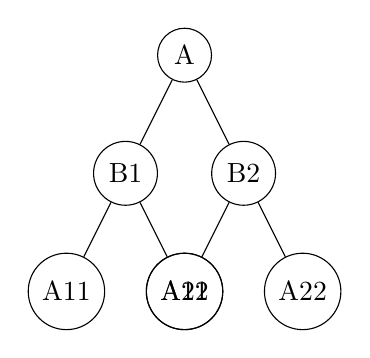
\begin{tikzpicture}
            \node[circle,draw](z){A}
            child{
                    node[circle,draw]{B1}
                    child{
                            node[circle,draw]{A11}
                        }
                    child{
                            node[circle,draw]{A12}
                        }
                }
            child{
                    node[circle,draw]{B2}
                    child{
                            node[circle,draw]{A21}
                        }
                    child{
                            node[circle,draw]{A22}
                        }
                };
        \end{tikzpicture}
    \end{center}
\end{figure}

\begin{definition}(Gioco in Forma Normale)
\end{definition}

Un gioco in forma normale è identificato da una tupla $<N,A,u$ dove:
\begin{itemize}
    \item $N = \{1,2,\dots,n\}$ giocatori
    \item $A = {A_1, A_2, \dots, A_n}$ insieme delle azioni disponibili per ogni giocatore
    \item $u = (u_1, u_2, \dots, u_n)$ dove $u_i: A \rightarrow \mathbb{R}$ è la funzione di payoff del giocatore $i$
\end{itemize}

\subsection{Giochi strategia puri}
In questo caso, assumiamo che \textit{il giocatore i conosca cosa gli altri
    giocatori giocheranno}.
\[
    a_i = <a_1,a_2,\dots,a_{i-1}, a_{i+1}, \dots, a_n>
\]

La \textbf{strategia migliore} per $a_i$ è quelal che massimizza il payoff:
\[
    a_i^* = FORMULA DA COPIARE
\]

\begin{definition}(Equilibro di Nash puro)
    Un profilo di azioni è un \textbf{Equilibro di Nash puro} se ogni giocatore giocasse la migliore azoine
\end{definition}

\[
    a = <a_1, a_2, \dots, a_n>  =  NE \iff \forall i a_i \in BR(a_i)
\]

\subsubsection{Dilemma del prigioniero}
\textbf{Idea del gioco}: Ogni giocatore ha un incentivo di scegliere una \textbf{soluzione sub-globale ottima}.

\begin{table}[H]
    \begin{center}
        \begin{tabular}{|c|c|c|}
            \hline
              & C   & D   \\
            \hline
            C & 3,3 & 0,5 \\
            \hline
            D & 5,0 & 1,1 \\
            \hline
        \end{tabular}
    \end{center}
\end{table}

\textbf{Spiegazione}: Se entrambi i giocatori scelgono C, ottengono un payoff di 3. Se entrambi scelgono D, ottengono un payoff di 1. Se uno sceglie C e l'altro D, il primo ottiene 0 e il secondo 5.
Ci sono molte strategie in gioci del genere, ad esempio tradire sempre, tradire al primo tradimento (che sembra la più funzionale).

\subsubsection{Pure Coordination}
Non ho capito: tipo se fai incidente non vieni pagato sennò si.
\begin{table}[H]
    \begin{center}
        \begin{tabular}{|c|c|c|}
            \hline
              & C   & D   \\
            \hline
            C & a,a & 0,0 \\
            \hline
            D & 0,0 & a,a \\
            \hline
        \end{tabular}
    \end{center}
\end{table}

\subsubsection{Battle of the Sexes}
Si ha una coppia di partner che vogliono vedere un film insieme. Si vede un
film Comedy o Action. Uno dei due vuole vedere Action, uno vuole vedere Comedy.
Se si vede il film da soli, non si ottiene una payoff. C'è una componente
egoistica: \textit{ognuno vuole vedere qualcosa che piace a lui}. In base a se
si sceglie $A$ o $C$, si ottiene una payoff sbilanciata, sempre.

\begin{table}[H]
    \begin{center}
        \begin{tabular}{|c|c|c|}
            \hline
              & A   & C   \\
            \hline
            A & 2,1 & 0,0 \\
            \hline
            C & 0,0 & 1,2 \\
            \hline
        \end{tabular}
    \end{center}
\end{table}

\textbf{Soluzione ipotetica:} Sarebbe quello di avere un 50\% di scelta di avere Comedy e 50\% Action \textbf{randomizzata}.

\subsubsection{Matching Pennies}
Sarebbe \textbf{testa o croce}. (H o T) Come si può vedere dalla tabella
\textbf{non c'è un equilibrio puro}. Il problema di questi giochi è che, in
alcuni, \textbf{non esiste} un equilibro puro.
\begin{table}[H]
    \begin{center}
        \begin{tabular}{|c|c|c|}
            \hline
              & H    & T    \\
            \hline
            H & 1,-1 & -1,1 \\
            \hline
            T & -1,1 & 1,-1 \\
            \hline
        \end{tabular}
    \end{center}
\end{table}

\textbf{La migliore strategia}: Letteralmente conviene randomizzare la scelta tra \textbf{testa} o \textbf{croce}, per massimizzare la payoff.

\subsection{Strategie e strategie miste}

\begin{definition}(Strategia)
\end{definition}

Una strategia $s_i$ per un giocatore $i$ è una \textbf{distribuzione di
    probabilità} su $A_i$.

\textbf{Strategia Pura:} Una sola azione viene giocata con probabilità 1.

\textbf{Strategia Mista:} Più di un'azione viene giocata con probabilità $> 0$.(Cioè non si ha una sola scelta che si fa per ogni mossa in ogni gioco). Le azioni con probabilità $>0$ vengono chiamate \textbf{supporto} della strategia.
\textbf{Nota:} con mosse con probabilità maggiore di 0 si indicano le possibili mosse da giocare.
Indichiamo $S_i$ l'insieme delle strategie del giocatore $i$.

Indichiamo con $S = S_1 \times S_2 \times \dots \times S_n$ l'insieme delle
strategie di tutti i giocatori.

\begin{domanda}(Come vengono calcolate le utilità nelle strategie miste?)
\end{domanda}

Siccome le mosse non sono stabilite, cioè non è solo una mossa, \textbf{non
    possiamo} usare la \textbf{payoff matrix}, perché stiamo introducendo le
\textbf{probabilità}. Ci vuole un altro modo per calcolarlo. Si utilizza
l'\textbf{utilità attesa}.

\begin{equation}
    \begin{aligned}
        u_{i(s)}= \sum_{\alpha\in A} u_{i(\alpha)}Pr(\alpha|s) \\
        Pr(\alpha|s) = \prod_{j \in N} s_j(\alpha_j)
    \end{aligned}
\end{equation}

\begin{esempio}(Testa o Croce)

\end{esempio}

\begin{table}[H]
    \begin{center}
        \begin{tabular}{|c|c|c|}
            \hline
              & H    & T    \\
            \hline
            H & 1,-1 & -1,1 \\
            \hline
            T & -1,1 & 1,-1 \\
            \hline
        \end{tabular}
    \end{center}
\end{table}

Considernado che ogni posizione della matrice ha una possibilità 0.5.
\[
    u_r(\big[\frac{1}{2}, \frac{1}{2}\big], \big[\frac{1}{2}, \frac{1}{2}\big]) = 1 \times 0.25 - 1 \times 0.25 - 1 \times 0.25 - 1 \times 0.25 = 0 \]

\begin{definition}(Migliore risposta con strategie miste)
    Supponiamo che il giocatore $i$ conosca cosa giocherà l'altro giocatore
    \[
        s_i = <s_1, s_2, \dots, s_{i-1}, s_{i+1}, \dots, s_n>
    \]

    La \textbf{migliore risposta con strategia mista} di $s_i$ è la strategia che
    massimizza il payoff del giocatore $i$.

    \[
        s_i^* \in BR(s_i) \iff \forall s_i \in A_i, u_i(s_i^*,s_{-i}) \geq u_i(s_i, s_{-i})
    \]
\end{definition}

\begin{definition}(Equilibro di Nash Misto)
    Un profilo strategico si definsice \textbf{Equilibro di Nash Misto} se ogni giocatore gioca la migliore risposta:

    \[
        s = <s_1, s_2, \dots, s_n> = NE \iff \forall i s_i \in BR(s_{-i})
    \]

    \textbf{Teorema:} Ogni gioco finito ha un Nash Equilibro.
\end{definition}

\subsection{Nash Equilibria}

\textbf{Condizione per migliore risposta}: Siano A e B le matrici di payoff for la riga e la colonna per players, rispettivamente.
Una strategia $s_r^*$ per la \textbf{giocatore riga} è la migliore risposta alla\textbf{ strategia della giocatore colonna} $s_c$ se e solo se:
\[
    s_{r,i}^* > 0 \implies (As_c^T)_i = \max(As_c^T) \forall i \in A_1
\]
\textbf{Nota:} $A_1$ è l'insieme di azioni del giocatore riga e $A_2$ è l'insieme di azioni del giocatore colonna.

Praticamente, ci dice che la \textbf{strategia migliore per il giocatore riga}
è quella che \textbf{massimizza} il \textbf{payoff} per ogni strategia del
giocatore\textbf{colonna}.

\begin{esempio} Sassa, carta o forbice
\end{esempio}

%matrice con 0 -1 1
%   1 0 -1
%  -1 1 0

%matrice matematica
$A = \begin{bmatrix}
        0  & -1 & 1  \\
        1  & 0  & -1 \\
        -1 & 1  & 0  \\
    \end{bmatrix}$


$s_c = \begin{bmatrix}
        \frac{1}{2} \\
        \frac{1}{2} \\
        0
    \end{bmatrix}$

%insert vector 1/2, 1/2, 0
$As_c^T = \begin{bmatrix}
        0  & -1 & 1  \\
        1  & 0  & -1 \\
        -1 & 1  & 0
    \end{bmatrix} \begin{bmatrix}
        \frac{1}{2} \\
        \frac{1}{2} \\
        0
    \end{bmatrix} = \begin{bmatrix}
        -\frac{1}{2} \\
        \frac{1}{2}  \\
        \frac{1}{2}
    \end{bmatrix}$

\textbf{Nota:} $As_c^T$ è il prodotto tra la matrice di payoff del giocatore riga e la strategia del giocatore colonna.


\begin{esempio}(Battle of Sexes)
\end{esempio}

$A = \begin{bmatrix}
    2 & 0 \\
    0 & 1 
\end{bmatrix} B = \begin{bmatrix}
    1 & 0 \\
    0 & 2 
\end{bmatrix} s_c = \begin{bmatrix}
    \frac{1}{2} \\
    \frac{2}{2} 
\end{bmatrix}
$

\textbf{Utilità giocatore colonna:} 
$
As_c^T = \begin{bmatrix}
    \frac{2}{3} & \frac{2}{3} 
\end{bmatrix}
$

\textbf{Migliore risposta:}

$s_r^* = \begin{bmatrix}
    1 \\
    0
\end{bmatrix}$





\begin{esempio}(Esempio con matrice)
\end{esempio}

%make font bigger for table
\renewcommand{\arraystretch}{2}

\begin{table}[H]
    \begin{center}
        \begin{tabular}{|c|c|c|}
            \hline
                  & $C_1$                                                    & $C_2$                                                    \\
            \hline
            $R_1$ & \textcolor{red}{\textbf{2}},\textcolor{blue}{\textbf{1}} & \textcolor{red}{\textbf{0}},\textcolor{blue}{\textbf{2}} \\
            \hline
            $R_2$ & 1,1                                                      & 1,3                                                      \\
            \hline
        \end{tabular}
    \end{center}
\end{table}

\textbf{Spiegazione}: Praticamente, se il giocatore usasse la strategia di $R_1$,
sceglierebbe quella \textbf{migliore}; in entrambi i casi, se il giocatore colonna usasse la colonna $C_1$ o $C_2$, il giocatore \textbf{riga} avrebbe un payoff maggiore rispetto ad usare la strategia di $R_2$. Quindi, la strategia migliore per il giocatore riga è quella di $R_1$.

\subsubsection{Giochi a Somma-Zero}

Siamo nel caso di giochi con $2$ giocatori.
\begin{definition}(Giochi a Somma-Zero)

    Un gioco con due giocatori (A,B) è definito a \textbf{somma-zero} se \textbf{A
        = -B}.

    Data una strategia $x$ dal giocatore riga, il giocatore colonna può scegliere
    una strategia $y$ che limita il payoff del giocatore riga.

    Inversamente, data una strategia $y$ del giocatore colonna, il giocatore riga
    punta a massimizzare la propria payoff.
\end{definition}

Formalizzazione sotto forma di \textbf{problema lineare}:

\begin{minipage}{0.5\textwidth}
    \textbf{Giocatore colonna:}

    \begin{equation}
        \begin{aligned}
            \min_{v,y} v       \\
            s.t.               \\
            Ay^T \leq \vec{1}v \\
            y \in S_2
        \end{aligned}
    \end{equation}
\end{minipage}
\begin{minipage}{0.5\textwidth}
    \begin{itemize}
        \item $v$: è il valore che il giocatore colonna vuole minimizzare
        \item $y$: è la strategia del giocatore colonna
        \item $Ay^T$: è la matrice di payoff del giocatore colonna
        \item $S_2$: è l'insieme delle strategie del giocatore colonna
    \end{itemize}
\end{minipage}

\begin{minipage}{0.5\textwidth}
    \textbf{Giocatore riga:}

    \begin{equation}
        \begin{aligned}
            \max_{u,x} u       \\
            s.t.               \\
            Ax^T \geq \vec{1}v \\
            x \in S_1
        \end{aligned}
    \end{equation}
\end{minipage}
\begin{minipage}{0.5\textwidth}
    \begin{itemize}
        \item $u$: è il valore che il giocatore riga vuole massimizzare
        \item $x$: è la strategia del giocatore riga
        \item $Ax^T$: è la matrice di payoff del giocatore riga
        \item $S_1$: è l'insieme delle strategie del giocatore riga
    \end{itemize}
\end{minipage}

\begin{esempio}(Esempio con Sasso Carta o Forbice)
\end{esempio}

\begin{equation}
    \begin{aligned}
        \max_{u,x} u \\
        s.t.         \\
        xA \geq \vec{1}u \\
        x \in S_1\\
    \end{aligned}
\end{equation}

\begin{center}
    
    $A = \begin{bmatrix}
        0 & -1 & 1 \\
        1 & 0  & -1 \\
        -1 & 1 & 0
    \end{bmatrix}
    $
\end{center}

\begin{equation}
    \begin{aligned}
        \max_{u,x} u \\
        0x_1 + 1x_2 - 1x_3 & \geq u \\
        -1x_1 + 0x_2 + 1x_3 & \geq u \\
        1x_1 - 1x_2 + 0x_3 & \geq u \\
        x_1 + x_2 + x_3 & = 1 \\
    \end{aligned}
\end{equation}

\textbf{Portare in forma normale}

\begin{equation}
    \begin{aligned}
        \min_{x} cx \\
        s.t.     \\
        M_{ub} x \leq b_{ub} \\
        M_{eq} x = b_{eq} \\
        x \geq 0 \\
    \end{aligned}
\end{equation}

\begin{equation}
    \begin{aligned}
        \min_{x} cx \\
        0x_1 - 1x_2 + 1x_3 1x_4 & \leq 0 \\
        1x_1 - 0x_2 - 1x_3 + 1x_4 & \leq 0 \\
        -1x_1 + 1x_2 + 0x_3 + 1x_4 & \leq 0 \\
        1x_1 + 1x_2 + 1x_3 + 0x_4 & = 1 \\
    \end{aligned}
\end{equation}

\begin{center}
    
    $M_{ub} = \begin{bmatrix}
        0 & -1 & 1 & 1 \\
        1 & 0 & -1 & 1 \\
        -1 & 1 & 0 & 1 \\
    \end{bmatrix}, b_{ub} = \begin{bmatrix}
        0 \\
        0 \\
        0 \\
    \end{bmatrix}
    $

    $M_{eq} = \begin{bmatrix}
        1 & 1 & 1 & 0 \\
    \end{bmatrix}, b_{eq} = 1, c = (0,0,0,-1)$
\end{center}
    
    




\begin{esempio}(Equilibrio Misto con 2 giocatori)
\end{esempio}

\begin{table}[h]
    \begin{center}
        %tabella    A   C
        %A 2,1 0,0
        %C 0,0 1,2
        \begin{tabular}{|c|c|c|}
            \hline
              & A   & C   \\
            \hline
            A & 2,1 & 0,0 \\
            \hline
            C & 0,0 & 1,2 \\
            \hline
        \end{tabular}
    \end{center}
\end{table}

Il giocatore 1 gioca A con probabilità $p$ e C con probabilità $1-p$

Il giocatore 2 cerca di rispondere al meglio al giocatore 1.

\textbf{Giocatore 2 rende il giocarore 1 indifferente tra A e C}

\begin{equation}
    \begin{aligned}
        u_1(A)      & = u_1(C)      \\
        2p + 0(1-p) & = 0p + 1(1-p) \\
        p           & = \frac{1}{3}
    \end{aligned}
\end{equation}

Il giocatore 1 gioca A con probabilità $q$ e C con probabilità $1-q$

Il giocatore 2 cerca di rispondere al meglio al giocatore 1.

\textbf{Giocatore 1 rende il giocatore 2 indifferente tra A e C}
\begin{equation}
    \begin{aligned}
        u_2(A)      & = u_2(C)      \\
        1q + 0(1-q) & = 0q + 2(1p)  \\
        q           & = \frac{2}{3}
    \end{aligned}
\end{equation}

Le strategie miste $\bigl(\frac{1}{3}, \frac{2}{3}\bigr)$ e $\bigl(\frac{2}{3},
    \frac{1}{3}\bigr)$ sono un \textbf{Equilibro di Nash}

